\begin{figure*}[!t]
\centering
\begin{minipage}[t]{\textwidth}
\noindent\begin{minipage}[t]{0.48\linewidth}
\vspace{0pt}\textbf{a}\quad Treatment compliance\par\smallskip
\noindent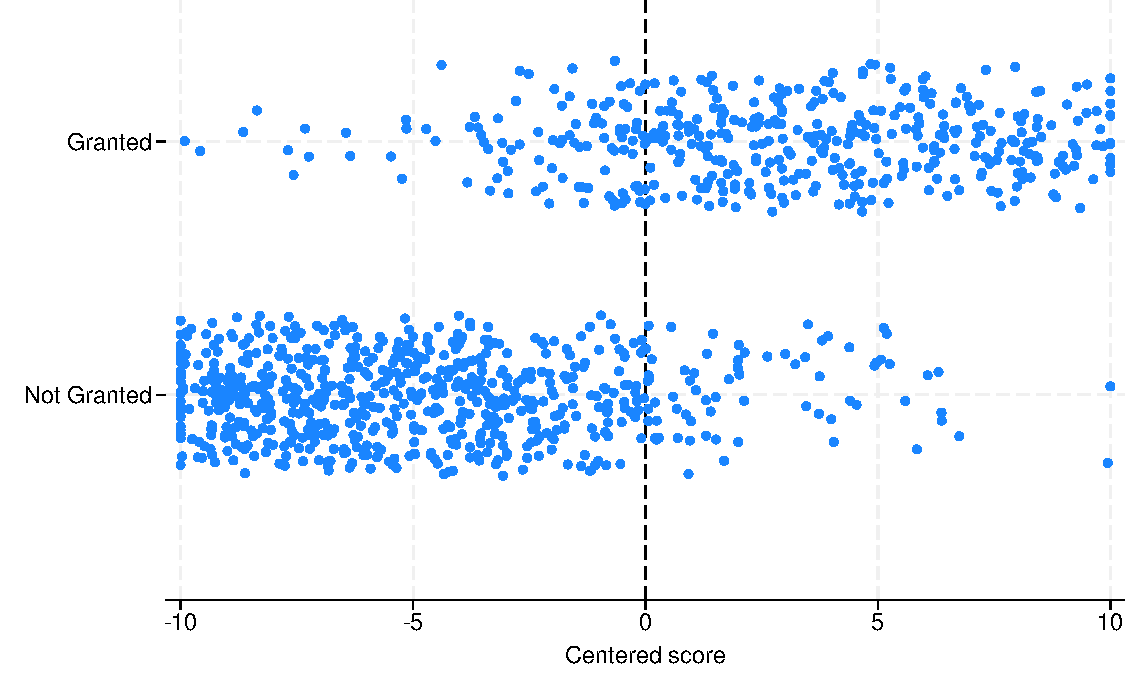
\includegraphics[width=\linewidth]{output/figures/figure1_compliance.pdf}
\end{minipage}\hspace{0.3cm}%
\begin{minipage}[t]{0.48\linewidth}
\vspace{0pt}\textbf{b}\quad Probability of receiving the grant\par\smallskip
\noindent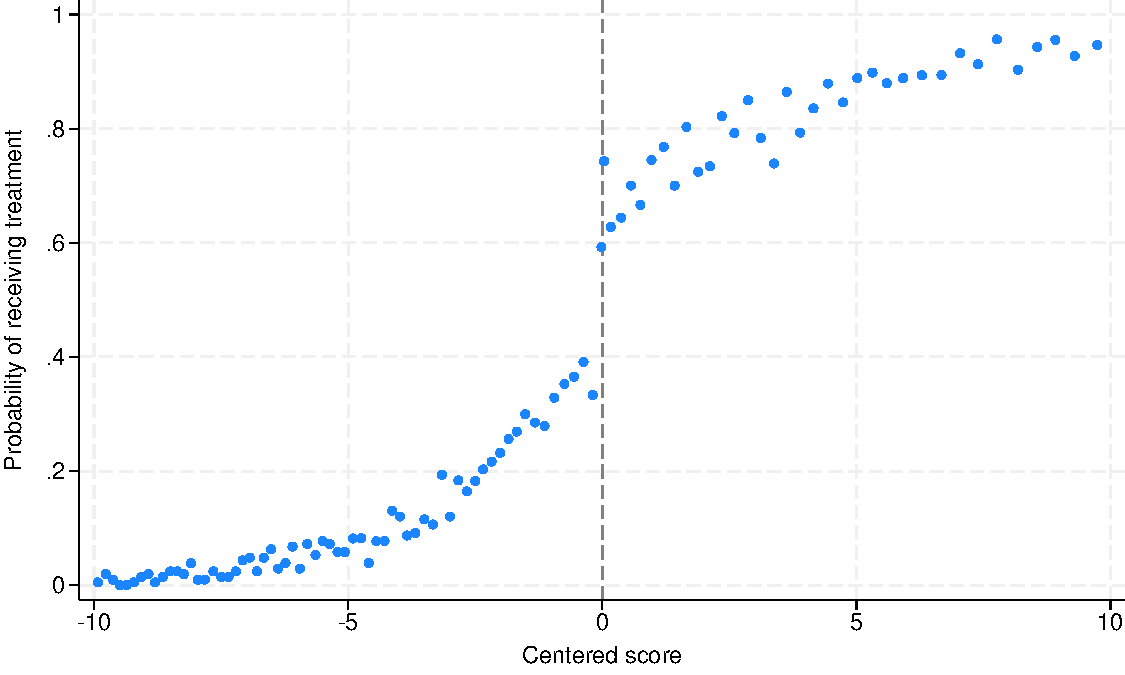
\includegraphics[width=\linewidth]{output/figures/figure1_probability.pdf}
\end{minipage}
\par\vspace{4mm}
\noindent\textbf{c}\quad Covariate balance around the funding threshold\par\smallskip
\noindent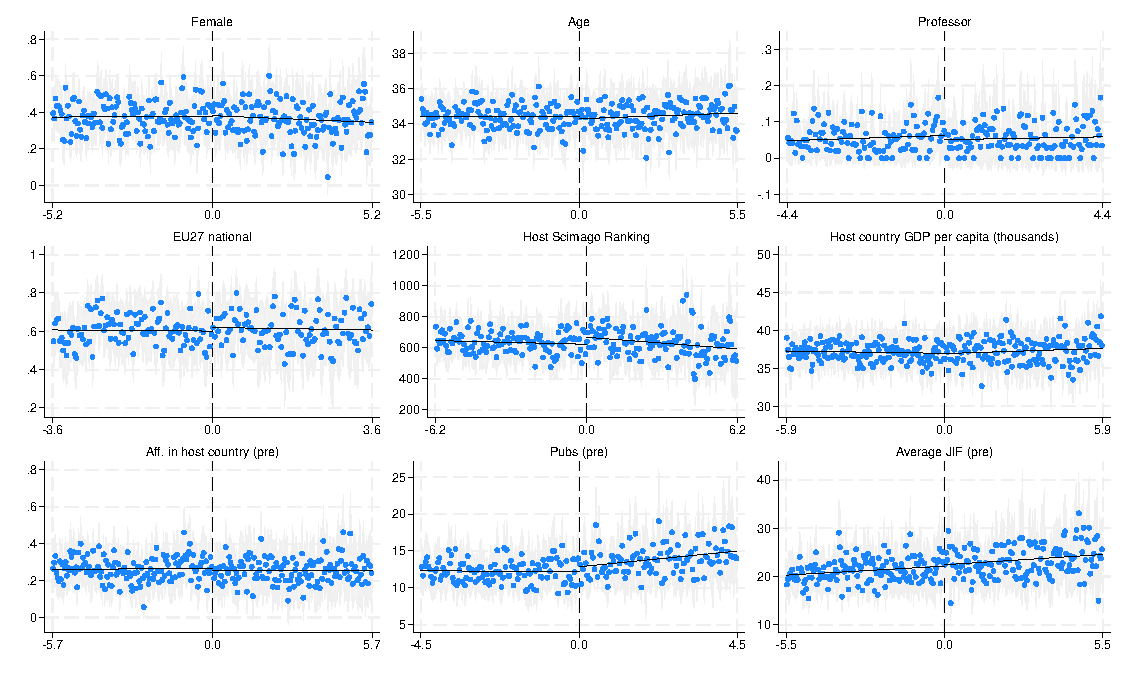
\includegraphics[width=\linewidth]{output/figures/figure1_balance.pdf}
\end{minipage}
\caption{\textbf{Funding thresholds, treatment compliance and covariate balance.} (a) Fifteen randomly selected competitions illustrate two-sided non-compliance in the vicinity of the funding threshold (-10,10): some applicants who are initially above the funding threshold and were offered the grant do not receive funding, whereas some applicants below the threshold do. (b) Relationship between centered score and award status in the vicinity of the funding threshold (-10,10). The probability of obtaining funding shows a clear jump around the funding threshold. (c) Pre-treatment applicant characteristics in the vicinity of the funding threshold. These plots show that applicants on either side of the threshold are similar. Bandwidths around the threshold are optimally selected for each covariate separately. Lines are local linear fits on either side of the cutoff using mean-squared-error-optimal bandwidths; shaded areas show 95\% confidence intervals. GDP per capita is displayed in thousands. Host rankings refer to 2013 Scimago Institutions Rankings.}
\label{fig:design}
\end{figure*}
